\chapter{Detection de region et de point d'intérêt dans les images}


\section{Detection de régions "gratuite" }

Des solution à base de réseaux à proposition de région (RPN) permettent une proposition automatique des régions par le réseaux. Ces approches ont montrés des résultats de l'état de l'art, comme montré dans la section (cite section). Ces approches permettent le developpement de réseaux comme Faster R-CNN ou plus récemment les Mask R-CNN, qui donnent les meilleurs résultats de l'état de l'art.

Ces genre de méthodes nécessite toutefois une base de données d'image annotées avec leur régions pour fonctionner. Nous ne visons pas une précision aussi élevé, et nous ne disposons pas d'une base de donnée annotée pour les images. Ceci nous amène à développer des solutions ne nécessitant pas la présence de boite englobante dans le corpus d'apprentissage.

Une première approches consiste à utiliser une base d'apprentissage différente au départ. Avec une base d'apprentissage de grande taille, il est possible d'entrainer un réseau de neurones très profond, avec les résultats de l'état de l'art. Comme montré dans la section (transfert learning), il est possible d'apprendre sur un corpus, et de faire un apprentissage fin sur le corpus final. Pour la détection de region, le même genre d'approche est possible. 

Dans CLEF2016, le réseau est appris sur une grande collection d'image, avec les objets bien identifiable. Ce réseau est ensuite utilisé sur les images cible, en passant le réseau de manière strié sur l'ensemble de l'image. Chaque zone de l'image est alors accompagné d'un activation du réseau. En prenant le maximum d'activation, il est possible de créer des zone d'activation correspondant aux différentes classes.

En appliquant cette approche à nos collection de test, nos obtenons les résultats présentés sur la figure~\ref{fig:heatmaps}. EXPLICATION FIGURE.

On remarque sur les carte d'activation que l'objet correspond à une zone d'activation élevé. Par contre, en regardant les labels, plusieurs objets différent peuvent être associé à cette région. On voit avec cette méthode les limites du transfert de connaissance. Ces résultats expliquant pourquoi un apprentissage fin sur une collection de petite taille ne permet pas d'avoir des résultats suffisant (section Expé). En revanche, cette méthode permet d'identifier les régions d'intérêt de l'image.




\begin{figure}
  \centering
  \begin{minipage}[c]{.33\linewidth}
    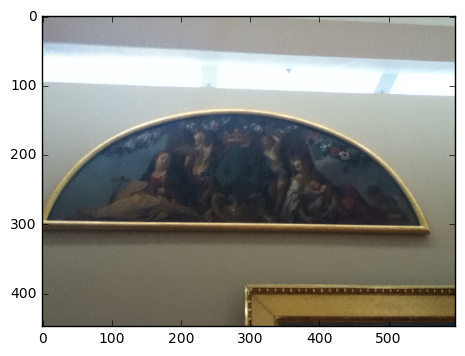
\includegraphics[width=\textwidth]{figures/sample1_10A-0519.png}
    %\caption{Image with label 10A\label{fig:sample1_id}}
  \end{minipage} \hfill
  \begin{minipage}[c]{.33\linewidth}
    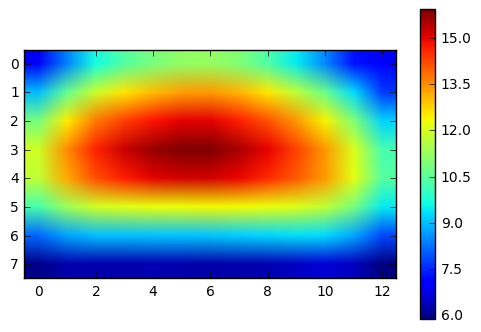
\includegraphics[width=\textwidth]{figures/sample1_heatmap.png}
    %\caption{Heat-map for 10A\label{fig:sample1_hm}}
  \end{minipage} \hfill
  \begin{minipage}[c]{.32\linewidth}
    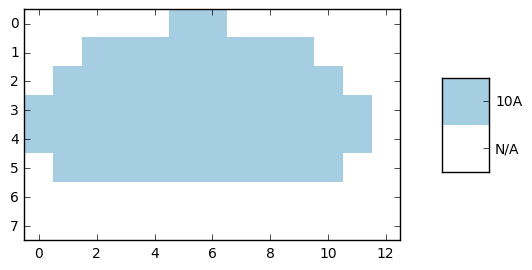
\includegraphics[width=\textwidth]{figures/sample1_labels.png}
    %\caption{Label-map for 10A\label{fig:sample1_lab}}
  \end{minipage}

  \begin{minipage}[c]{.33\linewidth}
    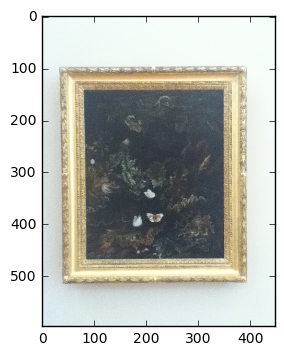
\includegraphics[width=\linewidth]{figures/sample2_5P-0508.png}
    %\caption{Image with label 5P\label{fig:sample2_id}}
  \end{minipage} \hfill
  \begin{minipage}[c]{.33\linewidth}
    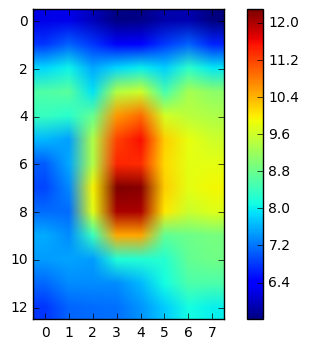
\includegraphics[width=\linewidth]{figures/sample2_heatmap.png}
    %\caption{Heat-map for 5P\label{fig:sample2_hm}}
  \end{minipage} \hfill
  \begin{minipage}[c]{.32\linewidth}
    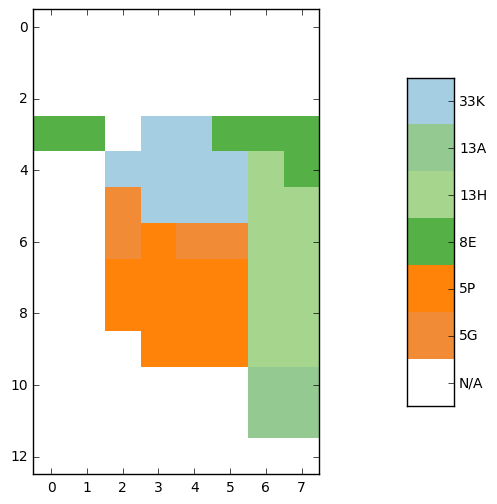
\includegraphics[width=\linewidth]{figures/sample2_labels.png}
    %\caption{Label-map for 5P\label{fig:sample2_lab}}
  \end{minipage}
  
  \begin{minipage}[c]{.33\linewidth}
    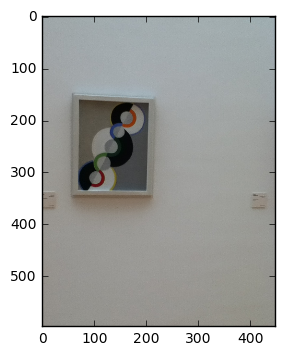
\includegraphics[width=\linewidth]{figures/sample3_30P-0976.png}
    %\caption{Image with label 30P\label{fig:sample3_id}}
  \end{minipage} \hfill
  \begin{minipage}[c]{.33\linewidth}
    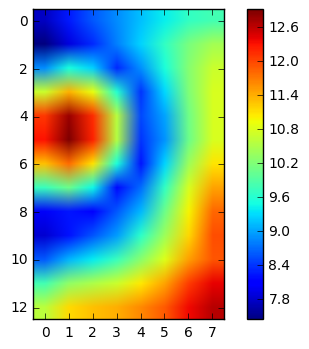
\includegraphics[width=\linewidth]{figures/sample3_heatmap.png}
    %\caption{Heat-map for 30P\label{fig:sample3_hm}}
  \end{minipage} \hfill
  \begin{minipage}[c]{.32\linewidth}
    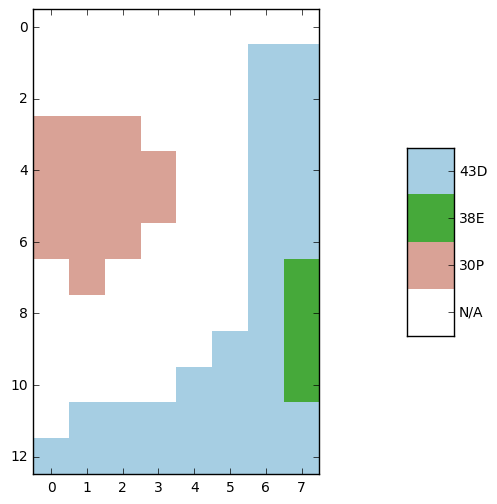
\includegraphics[width=\linewidth]{figures/sample3_labels.png}
    %\caption{Label-map for 30P\label{fig:sample3_lab}}
  \end{minipage}


	\caption{Exemple d'images avec les heat-map des activations maximales, obtenues à partir d'un ResNet-152 après un apprentissage fin. Le réseau est appliqué sur toute l'image de manière strié. Les labelles obtenu sur les zones d'activation maximales sont également indiqués.\label{fig:heatmaps}}
	
\end{figure}

Nous avons montré dans (section état de l'art), qu'un réseau entièrement convolutionel peut être appliqué sur une image quelque soit ça dimension. Cela permet d'appliquer un réseau de manière strié sur une grande image, sans faire plusieurs passage sur l'image.

Dans le but de faire un apprentissage fin, nous n'utilisons pas de réseau entièrement convolutionel, mais des CNN classique, avec couche de classification à la fin. Cependant, nous avons montré dans (section Etat de l'art) qu'il était possible de transformer une couche entièrement connecté, en une couche convolutionel. En utilisant cette méthode, il est possible d'obtenir les résultats présenté dans la figure~\ref{fig:heatmaps}, avec un réseau entièrement convolutionel.

Pour apprendre le réseau, nous utilisons le différentes échelles pour une image, et pour chaque échelle, différentes régions. La fonction de coût est calcul en moyennant l'entropie croisée, entre les régions, et entre les échelles. L'entropie croisée est calculée 


\begin{figure}
\centering
    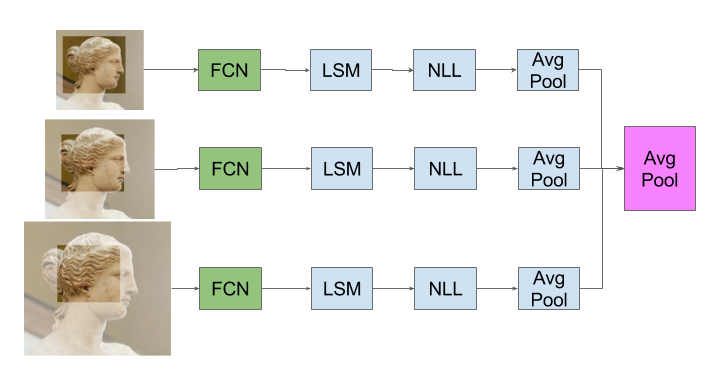
\includegraphics[width=\linewidth]{figures/Average_Loss.png}
    \caption{Calcul de la fonction de coût lorsque l'on entraine le réseau sur différentes régions à différentes échelles. LSM est le LogSoftMax et NLL le Negative Log-Likelihood. Il sont utilisés dans le calcul de la cross-entropy(eq.~\ref{eq:CE}).
    \label{fig:regionfinetuning}}
\end{figure}


\begin{equation}\label{eq:CE}
	\mathcal{CE}(x,y) = -y \log(softmax(x))
\end{equation}

\begin{equation}\label{eq:fcnloss}
 \mathcal{L} = \frac{1}{S} \sum_{s=1}^S \frac{1}{H_s*W_s}
\sum_{h=1}^{H_s} \sum_{w=1}^{W_s} \mathit{CE}^{h,w}
\end{equation}


Dans l'équation~\ref{eq:fcnloss}, $S$ est le nombre d'échelles de l'image de départ.
$H_s$ et $W_s$ représentent la hauteur et la largeur de la carte de caractéristiques (feature-map), à une échelle $s$ données.
$CE^{h,w}$ représente la cross-entropie pour une région $(h,w)$.



\section{Apprentissage des zones d'intérêt de l'image}



